%%%%%%%%%%%%%%%%%%%%%%%%%%%%
% Do Elections Affect Fed Forecasts?
% Cassandra Grafström and Christopher Gandrud
%%%%%%%%%%%%%%%%%%%%%%%%%%%%

% !Rnw weave = knitr

\documentclass[a4paper]{article}\usepackage{graphicx, color}
%% maxwidth is the original width if it is less than linewidth
%% otherwise use linewidth (to make sure the graphics do not exceed the margin)
\makeatletter
\def\maxwidth{ %
  \ifdim\Gin@nat@width>\linewidth
    \linewidth
  \else
    \Gin@nat@width
  \fi
}
\makeatother

\IfFileExists{upquote.sty}{\usepackage{upquote}}{}
\definecolor{fgcolor}{rgb}{0.2, 0.2, 0.2}
\newcommand{\hlnumber}[1]{\textcolor[rgb]{0,0,0}{#1}}%
\newcommand{\hlfunctioncall}[1]{\textcolor[rgb]{0.501960784313725,0,0.329411764705882}{\textbf{#1}}}%
\newcommand{\hlstring}[1]{\textcolor[rgb]{0.6,0.6,1}{#1}}%
\newcommand{\hlkeyword}[1]{\textcolor[rgb]{0,0,0}{\textbf{#1}}}%
\newcommand{\hlargument}[1]{\textcolor[rgb]{0.690196078431373,0.250980392156863,0.0196078431372549}{#1}}%
\newcommand{\hlcomment}[1]{\textcolor[rgb]{0.180392156862745,0.6,0.341176470588235}{#1}}%
\newcommand{\hlroxygencomment}[1]{\textcolor[rgb]{0.43921568627451,0.47843137254902,0.701960784313725}{#1}}%
\newcommand{\hlformalargs}[1]{\textcolor[rgb]{0.690196078431373,0.250980392156863,0.0196078431372549}{#1}}%
\newcommand{\hleqformalargs}[1]{\textcolor[rgb]{0.690196078431373,0.250980392156863,0.0196078431372549}{#1}}%
\newcommand{\hlassignement}[1]{\textcolor[rgb]{0,0,0}{\textbf{#1}}}%
\newcommand{\hlpackage}[1]{\textcolor[rgb]{0.588235294117647,0.709803921568627,0.145098039215686}{#1}}%
\newcommand{\hlslot}[1]{\textit{#1}}%
\newcommand{\hlsymbol}[1]{\textcolor[rgb]{0,0,0}{#1}}%
\newcommand{\hlprompt}[1]{\textcolor[rgb]{0.2,0.2,0.2}{#1}}%

\usepackage{framed}
\makeatletter
\newenvironment{kframe}{%
 \def\at@end@of@kframe{}%
 \ifinner\ifhmode%
  \def\at@end@of@kframe{\end{minipage}}%
  \begin{minipage}{\columnwidth}%
 \fi\fi%
 \def\FrameCommand##1{\hskip\@totalleftmargin \hskip-\fboxsep
 \colorbox{shadecolor}{##1}\hskip-\fboxsep
     % There is no \\@totalrightmargin, so:
     \hskip-\linewidth \hskip-\@totalleftmargin \hskip\columnwidth}%
 \MakeFramed {\advance\hsize-\width
   \@totalleftmargin\z@ \linewidth\hsize
   \@setminipage}}%
 {\par\unskip\endMakeFramed%
 \at@end@of@kframe}
\makeatother

\definecolor{shadecolor}{rgb}{.97, .97, .97}
\definecolor{messagecolor}{rgb}{0, 0, 0}
\definecolor{warningcolor}{rgb}{1, 0, 1}
\definecolor{errorcolor}{rgb}{1, 0, 0}
\newenvironment{knitrout}{}{} % an empty environment to be redefined in TeX

\usepackage{alltt}
\usepackage{fullpage}
\usepackage[authoryear]{natbib}
\usepackage{setspace}
    \doublespacing
\usepackage{hyperref}
\hypersetup{
    colorlinks,
    citecolor=black,
    filecolor=black,
    linkcolor=cyan,
    urlcolor=cyan
}
\usepackage{dcolumn}
\usepackage{booktabs}
\usepackage{url}
\usepackage{tikz}
\usepackage[utf8]{inputenc} 

%%%%%%% Title Page %%%%%%%%%%%%%%%%%%%%%%%%%%%%%%%%%%%%%%%%%%%%
\title{Does Presidential Partisanship Affect Fed Inflation Forecasts?}

\author{Christopher Gandrud \\
                {\emph{Yonsei University}}\footnote{\href{mailto:gandrud@yonsei.ac.kr}{gandrud@yonsei.ac.kr}} \\
                and \\
            Cassandra Grafstr\"{o}m \\
                {\emph{University of Michigan}}\footnote{\href{mailto:cgrafstr@umich.edu}{cgrafstr@umich.edu}}}

\begin{document}



\maketitle

%%%%%%% Abstract %%%%%%%%%%%%%%%%%%%%%%%%%%%%%%%%%%%%%%%%%%%%
\begin{abstract}
\noindent\emph{Very Early draft version. Comments welcome.} \\[0.2cm]
Recent work argues that the Federal Reserve is not politically indifferent \citep{Clark2011}. The Fed tends to choose looser monetary policies during Republican administrations, possibly in order to ensure the (re)election of ideologically preferred administrations. This model excludes an essential aspect of monetary policy decision-making: expectations about future inflation. We use the Fed's Green Book forecasts to test whether the partisanship of a government shape the estimates of future economic performance that influence FOMC policies. We find that Federal Reserve staff probably do not bias their forecasts to influence Fed governors around elections. However, they do systematically overestimate inflation during Democratic presidencies and underestimate inflation during Republican ones. This suggests that while not electorally motivated, Fed staff have a partisan bias when making inflation forecasts.

\end{abstract}

\begin{description}
  \item [{\textbf{Keywords:}}] forecast bias, Federal Reserve, rational partisan cycle,
\end{description}

\vspace{0.3cm}

Recent work argues that the Federal Reserve is not politically indifferent \citep{Clark2011}. The Fed tends to choose looser monetary policies during Republican administrations, possibly to ensure the (re)election of ideologically preferred administrations. This bias is assumed by Clark and Arel-Bundock to arise from a Board of Governors that prefer rightist presidents to leftist ones and so set interest rates to help Republican incumbents and hinder Democratic ones. 

However, the Board of Governors makes monetary policy based on information provided to them by Federal Reserve staff about the future of the economy. If Fed staff expect higher inflation under Democrats than Republicans, these beliefs would be incorporated into the forecasts used by the Board of Governors to make policies. Thus partisan bias on the part of the Board of Governors is not necessary to produce the partisan cycles in interest rates observed in \cite{Clark2011}. 

We provide evidence that Fed internal forecasts of inflation consistently predict that inflation will be lower than it turns out to be under Republican presidencies and predict that inflation will be higher than it turns out to be under Democratic administrations. Even accounting for changes in monetary policy, Federal Reserve economists over-shoot inflation for Democrats and under-shoot for Republicans. We expound a partisan heuristic model of policy expectations that explains these predictive failures.

In this paper we first provide a brief discussion of what inflation forecasts and forecast errors are, including their importance for monetary policy making and our current understanding of how they are made. As we demonstrate in this first section, academic scholarship up till now has not examined possible partisan causes of forecast errors. We then introduce the issues of inflation forecast partisan biases and posit a number of ways that Green Book forecasting may be influenced by them. We test these theories with a series of regression models using both unmatched and matched data on Green Book inflation forecast errors from the 1970s through 2005. The models suggest that, even when controlling for a number of important economic and political factors, Green Book forecasts show a distinct presidential partisan bias. 

%%%%%%%%%%%%%% Section 1: Forecasting Inflation at the Fed %%%%%%%%%%%%%%%%%%%%%

\section{Forecasting Inflation at the Fed \& Inflation Forecast Errors}

In this section we briefly describe what Green Book inflation forecasts and forecast errors are, why they are an important part of monetary policymaking in the United States, and the current understanding of how Federal Reserve inflation forecasts were made since the late 1960s.

\subsection{Forecasting \& Forecasting Errors}
Prior to every meeting of the Federal Open Market Committee (FOMC - the primary policy-making body of the Federal Reserve)Federal Reserve staff create a document called the ``Current Economic and Financial Conditions" or ``Green Book" that contains information on recent behavior and forecasts of various macroeconomic aggregates. \footnote{Green Book data can be found at {\url{http://www.phil.frb.org/research-and-data/real-time-center/greenbook-data/philadelphia-data-set.cfm}}. Accessed December 2011.} The Federal Reserve staff produces forecasts of various elements of the US and global economies so that the FOMC can produce policies appropriate to fulfill the Fed's dual mandate of maintaining output growth and price stability. We focus on GNP/GDP price index forecasts in our study.\footnote{Note: GNP was used through 1991 (inclusive) and GDP was used from 1992 onward. Furthermore, the implicit deflator was used before the second quarter of 1996 and chain-weighted price index was used from the second quarter of 1996 onwards.} The FOMC uses these forecasts to determine the appropriate monetary policy to puruse. Higher inflationary expectations increase the likelihood of the FOMC tightening policy in order to slow inflation and an overheating economy; low inflationary expectations increase the likelihood of a loosening of monetary policy to bolster growth and employment, \emph{ceteris paribus}. 

Green Book forecasts are available for each quarter from the fourth quarter of 1964 through the end of 2005\footnote{There is a five year lagged release schedule.}. It is important to note that finalized forecasts of macroeconomic aggregates are a combination of both econometric models and the professional opinions of forecasters about likely changes in the economy's trajectory not necessarily picked up in these models \citep{Karamouzis1989,Reifschneider1997}. The forecasts contained in the Green Book are the ``consensus" forecasts combining {\bf{both}} econometric models and judgmental forecasts assuming current monetary policies remain unchanged. Below we briefly explain how the econometric aspects of these ``consensus" forecasts have been modeled.

\subsection{Our Current Understanding of Fed Inflation Forecasting}

The Federal Reserve produces forecasts of various elements of the US and global economies in order to formulate policies appropriate to fulfill the Fed's dual mandate of maintaining output and price stability.\footnote{This subsection draws heavily on Brayton et al.'s\nocite{Brayton1997} (1997) detailed description of the changes to Federal Reserve forecasting models that took place in 1996. See Brayton et al. 1997 for further details.} There have been two essential sets of econometric models used during our observation period. This section describes these two models and their importance for our understanding of forecast errors. It is important to note that finalized forecasts of macroeconomic aggregates are a combination of both these mathematical models \emph{and} the professional opinions of forecasters about likely changes in the economy's trajectory not necessarily picked up in these models \citep{Karamouzis1989,Reifschneider1997}. The most significant change with the move to the Federal Reserve Board (FRB) Models in the mid-1990s was the incorporation of rational, as opposed to adaptive, expectations by market actors. We discuss the early and current models followed by the implications each has for predicted forecast errors.

\paragraph{Early models of the economy}
The first simultaneous equation model of the US economy was developed and adopted by the Federal Reserve between 1966 and 1975. The model, originally developed in conjunction with MIT, University of Pittsburg, and the Social Science Research Council (MPS), was based on a neo-classical growth model of production and factor demands and embraced the IS/LM/Phillip's Curve paradigm. This model was composed of more than XYZ equations modeling various interdependent aspects of the American economy in a simultaneous equations framework. Homogeneity assumptions ensured neutrality of money in the long-run--that is, changes in the stock of money only affects nominal variables in the economy such as wages or prices but these changes have no effect on real (inflation adjusted) variables like real GDP or employment in the long-run because any increase in the money supply will be offset by a proportional increase in prices and wages eventually. The essential feature of this model, however, was that the public held {\bf{adaptive expectations}}. Basing a model off of adaptive expectations means that people's expectations abut what will happen in the future is based on what happened in the past. These models simply extrapolated future behavior of the economy from its recent past behavior, taking no account of the fact that people may change their behavior in response to future expected outcomes.

The collapse of Bretton Woods spurred a number of changes to the model. First, following the introduction of floating exchange rates the trade and exchange rate sections of the domestic economy were expanded significantly. Second, and more significantly, an explicit model of the global economy was developed. The Multi-Country Model (MCM) introduced in 1975 originally included estimates of macroeconomic performance in the US, Canada, Germany, Japan, the UK, and "the rest of the world sector." This model, which included both estimates of American consumption and production but then fed into equations of American consumption and production. This model was again based on the short-run dynamics of of the IS/LM/Phillip's Curve and long-run neo-classical growth model.

Both the MPS and MCM models were tweaked during the 1980s, with about one-third of the equations in the MPS model changed during this time. The MCM was also expanded to include a larger set of major trading partners.\footnote{The post-1992 model included each of the G-7 countries individually as well as Mexico, and blocks representing the OECD, newly industrialized countries, OPEC, and the rest of the world.} However, the basic assumptions of the models, specifically the adaptive expectations assumptions, remained unchanged. The exclusive use of VAR models (solely backwards looking actors) meant that the models failed to account for actors concerns about future outcomes explicitly in these models. The rational expectations revolution in economics in the 1970s and 1980s made this assumption an increasingly controversial one. Thus, the development of new models began in earnest in 1991.
 
\paragraph{Current models of the economy}
New models of the American economy's near-term trajectory replaced the MPS in 1997. The Federal Reserve Board US model (FRB/US) is composed of approximately 40 behavioral equations, estimated with single-equation techniques. This model explicitly considers the role of economic expectations in economic behavior. The foundational assumption of apadtive expectations in the old MPS model was thus replaced with {\bf{rational}} or {\bf{model-consistent expectations}}. In these models, prices are sticky and aggregate demand determines short-run output. Further, monetary policy's effects on the economy are extensively modeled. 

The Federal Reserve Board Global (FRB/Global) model's development began in 1993 and had replaced the MCM by 1996. The FRB/Global model links the behavioral equations of FRB/US with approximately 200 behavioral equations representing the other 11 regions of the model. Anticipated values of future variables directly influence interest and exchange rates, components of aggregate demand, and wages and prices.

\paragraph{Models and their effects on predicted forecast errors}
The innovations in how the Federal Reserve Board generates estimates of future economic performance (including changes to how they incorporated the effects of expected Fed interest rate policies has one important implication for forecast errors. Most notably, the move to rational expectations ought to shrink errors relative to the earlier period. The goal of incorporating forward looking actors into the models was to account for an important source of endogeneity in the earlier models that would lead to overestimates of important economic indicators under some circumstances and underestimates of those same indicators under others. None of these over- or under-estimates, however, ought to have been linked to the party of the president. We would, however, expect that forecast errors' absolute magnitude will be smaller after 1996 than in the earlier era.

%Random thought: what if the models assume that voters have partisan expectations and behave according to those partisan characteristics. Then when the partisans fail to do so or when voters react to these as they should (by not reacting) this results in over or under-shooting inflation by the Fed, particularly under the early model?

\subsection{Forecast accuracy}

It is the accuracy of these forecasts that is of interest in this study. We measure accuracy as the forecast error,  calculating {\bf{forecast error}} $E$ as the difference between the Green Book inflation forecast $F$ for a given quarter $q$ and actual inflation $I$ as a proportion of actual inflation
%
\begin{equation}
    E_{q} = \frac{F_{q} - I_{q}}{I_{q}}
\end{equation}
%

We put the error in terms of actual inflation to control for the fact that mean actual inflation varies considerably across different periods (see Figure \ref{absolute}). An error of one percentage point is a significantly larger mistake when inflation is running at 3\% than when it is running at 13\%. Further, this measure allows us to incorporate forecasts from both the pre- and post-1997 era into a single model when we would expect systematically smaller errors in the latter period due to changes in how the Fed estimated inflation. 

If the forecasts are unbiased then the mean error of the forecasts would be indistinguishable from zero. While the Federal Reserve's internal forecasts meet this requirement over very long spans of time \citep{Romer2000}, long periods of over- or under-predicting inflation can be seen in Figure \ref{absolute} \citep{Capistran2006}. Within economics the Fed's forecasts have been examined for evidence of rationality. These studies have rarely incorporated political preferences of the Fed because Federal Reserve staffers are assumed to be politically independent, even if the voting behavior of the FOMC members may not be \cite{Clark2011}.

We have 161 forecast quarters in our data set, spanning the first Green Book's production in June 1964 through the end of 2005. Forecasts correspond to the FOMC meeting closest to the middle of the quarter. For a given quarter the data includes forecasts made in the present quarter and up to 5 quarters before. Actual inflation corresponding to each of these quarters\footnote{Inflation was calculated by comparing quarters year-on-year. The exact inflation measure that the Federal Reserve was forecasting changed a number of times, so the measure of actual inflation used to created the forecast error variable changes accordingly. The GNP deflator indicator is used from the beginning of our sample through the end of 1991. From the first quarter of 1992 through the first quarter of 1996 actual inflation is measured with the GDP deflator.  From the second quarter of 1996 we use the chain-weighted GDP price index. } was found using data from the Federal Reserve's FRED website.\footnote{See \url{http://research.stlouisfed.org/fred2/}. Accessed December 2011.} Absolute actual inflation for each quarter and inflation forecasts made two quarters before are compared in Figure \ref{absolute}. In general we use forecasts made two quarters before.\footnote{Using these two quarter forecasts constricts our observations to 150 since, apart from the first quater of 1968, two quarter forecasts are not included in the Green Book data before the fourth quarter of 1968.} 


%%%%%%%%%%%%%%%%%%%%%%%%%%  Raw Green Book estimate vs. actual graph
\begin{figure}[t]
    \caption{Green Book Inflation Forecasts and Actual Quarterly Inflation}
    \label{absolute}
    \begin{center}
    
\begin{knitrout}
\definecolor{shadecolor}{rgb}{0.969, 0.969, 0.969}\color{fgcolor}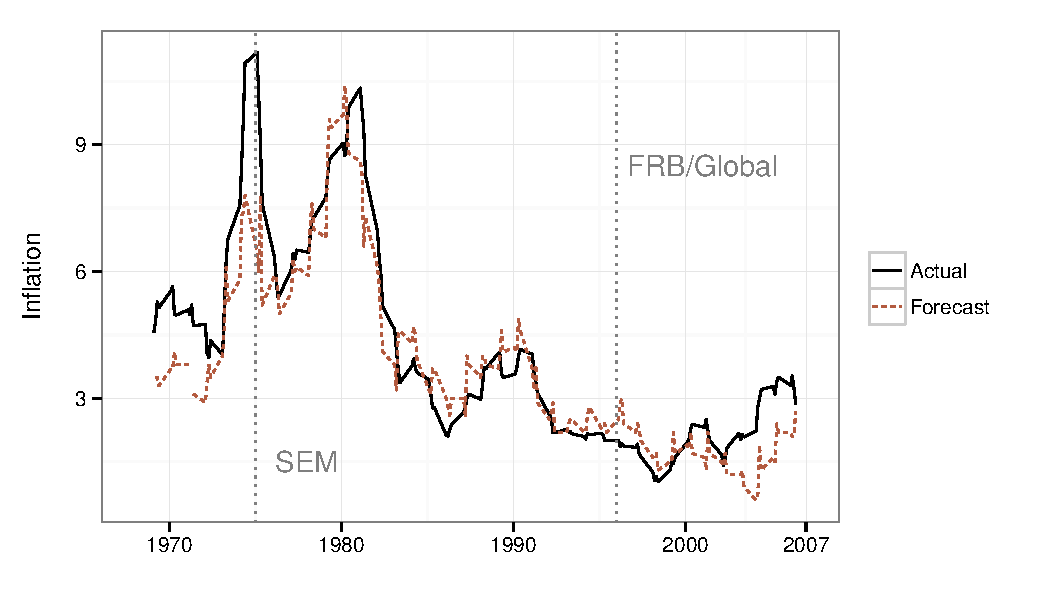
\includegraphics[width=0.8\linewidth]{figure/BaseInflation} 
\end{knitrout}

    
    \end{center}
    \begin{singlespace}
        {\scriptsize{Forecasts were made two quarters beforehand. \\
                     The grey dotted lines indicate the {\emph{approximate}} years that the Simultaneous Equation Models (SEM) and Federal Reserve Board Global (FRB/Global) forecasting models were fully implemented.  
                      }}
    \end{singlespace}
\end{figure}



\subsection{Partisan Forecast Errors}

As stated above, ideally forecasts should be unbiassed in that they have a mean error of zero \citep[5]{Bruck2006}. Using this criteria, forecasts errors should be the same--ideally with a mean of 0--regardless of the incumbent president's party identification. Looking only at forecast errors and the United States president's partisan identity, is it plausible that there is a partisan bias to Green Book inflation forecasts? Figure \ref{errors_over_time} plots forecast errors across our sample. We've shaded out errors made between $+/- 10$ percent of actual inflation. These could be considered largely random errors. 

The first thing to note is that inflation was almost never underestimated during the three Democratic presidential terms in our sample. Also, the largest overestimates were made during Clinton's (Democratic) presidency. All of the major inflation underestimates were made during Republican presidencies, particularly during Nixon's, Ford's, and George W. Bush's presidencies. Inflation was often overestimated during the second part of Reagan's first term, his second term and George H.W. Bush's term. Though it is important to note that over this period--often referred to as the Volker Revolution \citep[see][]{Bartels1985}--inflation was much lower than before, as we can see in Figure \ref{absolute}.

This summary examination of inflation forecast errors suggests that there might be partisan biases. Before jumping into a further empirical investigation of these errors, we discuss why we might expect the Fed to experience partisan bias.

%%%%%%%%%%%%%%%%%%%%%%%%%%   Green Book Error Across Time
\begin{figure}[t]
    \caption{Inflation Forecast Errors (1969 - 2005)}
    \label{errors_over_time}
    \begin{center}
    
\begin{knitrout}
\definecolor{shadecolor}{rgb}{0.969, 0.969, 0.969}\color{fgcolor}\includegraphics[width=0.8\linewidth]{figure/PartisanError} 
\end{knitrout}

    
    \end{center}
    \begin{singlespace}
        {\scriptsize{Note: An error of 0 indicates that inflation was perfectly forecasted. \\
            The grey shaded box indicates minimal error, i.e. $+/- 0.1$.
        }}
    \end{singlespace}
\end{figure}




%%%%%%%%%%%%%%%%%%%%%%%%%%%%% Section 2: Partisan Biases in Fed Inflation Forecasts? %%%%%%%%%%%%%%%%%%%%
\section{Partisan Biases in Fed Inflation Forecasts?}

In this section we try to understand trends in Fed inflation forecast errors by first discussing changes the economic models the staff used as part of the forecasting process. We then discuss theories from the the political economy literature that provide alternative explanations of why forecasts seem to have a partisan bias.

% This is basically the rational expectations lit. review section. Also propose a signalling game, i.e. biases part of Fed Staff trying to influence interest rate decisions around elections (i.e. its not the FOMC, its the Staff).

%%%%%%%%%%%%%%%%%% Section 3: Research Methods %%%%%%%%%%%%%%%%%%

\section{Research Methods}

We use non-matched and matched data sets with a number of parametric models \citep[see][]{Ho2007} to assess whether or not there are partisan biases in Green Book forecasts. This section discusses the choice of methods and variables. The following section discusses our results.

\subsection{Matching \& Models}

We are interested in disentangling the effects of presidential party ID and elections from the many background factors, such as economic shocks and FOMC policy changes, that might create inflation forecast errors. We treat presidential partisan identification and elections as `treatments'. Democratic presidencies are considered to be treatments. Republican presidencies are `controls'. The election quarter when an election is held and the quarter before it are considered treatments and all other quarters are controls. Of course, given that we are working with observational data, other variables that have an impact on forecast errors may have different distributions across the treatment and control groups \citep{Diamond2012, Cochran1973}. This makes it difficult to identify the relationships between presidential party ID, elections and errors from all of the confounding background variables.

To address this issue we follow the advice of \cite{Ho2007} to preprocess our data with matching to create data sets where the distributions of confounding variables are more even across treatment and control groups. We then run our parametric analyses with the matched data sets. To do this we used the {\tt{R}} package {\tt{MatchIt}} \citep{matchit2011} to create two matched data sets where the non-treatment covariates in the control groups closely matched with those in the treatment groups. Doing this helps us isolate the effects of these two `treatments' from that of the background covariates. 

Formally, each unit $i$ in the data set is `assigned' to either the treatment group ($t_{i} = 1$) or the control group ($t_{i} = 0$). $y_{i}(1)$ is the potential outcome--in our case the inflation forecast error-for unit $i$ of being in the treatment group, regardless of whether or not it was observed to be in this group. $y_{i}(0)$ is the potential outcome if $i$ was not in the treatment group, regardless of its observed assignment. It is impossible to observe both $y_{i}(1)$ and $y_{i}(0)$ at the same time. Instead we observe one version of $y_{i}=t_{i}y_{i}(1)-(1-t_{i})y_i{0}$. For each $i$ there is a fixed vector of exogenous confounders $X_{i}$. Ideally $t_{i}$ and $X_{i}$ are independent. However, this is not necessarily the case. The point of matching is to reduce or eliminate the relationship between $t_{i}$  and $X_{i}$ by selecting, dropping, and/or duplicating data. Ideally this process matches one treated unit with one controlled unit that has the same values of $X_{i}$, i.e. the distribution of covariates is the same in the treated and control groups \citep{matchit2011}. This is know as ``covariate balance" \cite[1]{Diamond2012}. Using matching to balance a data set ``break[s] the link between the treatment variables and the pre-treatment controls", effectively replicating the conditions of a randomized experiment with observational data \cite[][2--3]{matchit2011}. 

Balance is usually achieved in matching through propensity scores; the probabilities that unit were assigned the treatment given the covariates. The propensity score model is generally unknown \cite{Drake1993}. To find the propensity score model we use Diamond and Sekhon's \citeyearpar{Diamond2012} genetic matching method (GenMatch).\footnote{The method is implemented with {\tt{MatchIt}} The original source code for the exact matching models can be found at {\url{https://github.com/christophergandrud/GreenBook/blob/master/Analysis/MainAnalysis2.R}}.} GenMatch uses an evolutionary search algorithm to automate the search for the propensity score model that creates maximum balance.


\subsection{Parametric Models}

Once we had created our matched data sets we used two types of parametric models to examine the effects of our treatment variables on the continuous inflation forecast error. The first was ordinary least squares linear regression (i.e. OLS).\footnote{In {\tt{Zelig}} this is the {\tt{ls}} model.} The other type was Bayesian normal linear regression\footnote{In {\tt{Zelig}} this is the {\tt{normal.bayes}} model.} which is particularly useful for our limited sample as it makes ''valid small sample inferences via draws from the exact posterior" \citep[][38]{Zelig2012}. Please see the {\tt{Zelig}} manual for details about Bayesian normal linear regression \citep{Goodrich2007}.  See also \cite{Imai2008} for a discussion of how to combine nonparametric matching and parametric analysis in one research process. Because we used nonparametric matching methods, not only do we better isolate the treatments' effect from those of the background variables, but we also reduce our estimated causal effects' dependence on the type of model we choose \cite[200--201]{Ho2007}.

Our generic parametric model we used is given by
%
\begin{equation}
    E_{q} = \alpha + \beta T_{q} + \beta X_{q} + \epsilon,
\end{equation}
%
where $T_{q}$ is the treatment for quarter $q$ and $X$ is a vector of covariates. 

\subsection{Variables}

In Section 1 we discussed our dependent variable--inflation forecast errors. We are interested in seeing how US presidents' partisan identity and the existence of an upcoming presidential election affect these errors. So, we created {\bf{president party identification}} and {\bf{election period}} variables. The president party ID variable is 1 when the president is a Democrat and 0 when they are a Republican. Since forecast error data is released on a quarterly basis, we consider a president to be sitting from the first quarter after the election.\footnote{Elections are held almost at the midpoint--early November--of an election year's fourth quarter. Presidents are sworn into office near the beginning--20 January--of the following year's first quarter.} We consider quarters to be in the election period either if the presidential election is held in that quarter or the quarter before.\footnote{If $q_{e}$ is a quarter with an election then we code quarters $q_{e}$ and $q_{e-1}$ election quarters.}

To further examine whether or not Federal Reserve staff were taking into consideration an electoral business cycle, we include a variable of the {\bf{quarters until the presidential election}}. This simply counts down from the quarter after the previous election.\footnote{There are 15 quarters before a United States presidential election quarter.} The quarters that included presidential elections were coded as 0. 

The United States president does not set the level of government expenditure--one of the main non-monetary policy causes of inflation--by themselves. Instead, the president is constrained by the two houses of Congress. To examine whether or not Federal Reserve staff are taking into consideration the partisan composition of Congress as well as the president's party identification, we include variables of {\bf{Democratic legislators as a proportion of Republican legislators}} in the House of Representatives and the Senate. Data on the number of legislators with Republican and Democratic party IDs was found at infoplease.\footnote{See {\url{http://www.infoplease.com/ipa/A0774721.html}}. Accessed May 2012.} 

There are at least three possible ways that Congressional party identification may affect forecast errors. The first is a simple circumstance where Federal Reserve staff with rational partisan expectations pay attention to the partisan control of a chamber of Congress {\emph{independent of}} the president's party identification.  For example, Fed staff could predict higher spending if Democrats control one of the houses of Congress even if they do not control the other house or the presidency compared to a situation where all parts of the executive and legislature were controlled by Republicans. This might lead to higher inflation error.

Though they make different predictions, both of the latter two ways that partisan control of Congress may affect inflation forecasts are through interactions with presidential party identification.

The first interaction theory is that Federal Reserve staff with simple rational partisan expectations would presumably expect that a Democratic president would be able to get policies closer to their ideal point when there is a Congress with similar preferences. If a Democratic president had chambers of Congress controlled by Democrats, presumably Federal Reserve staff would expect even higher fiscal expenditures and therefore even higher inflation. Conversely, Republican presidents with a Republican-controlled Congress may be even better at cutting spending, leading to lower inflation.

The second interaction possibility is based largely on Krause's \citeyearpar{Krause2000} work about the affect of partisan divisions on fiscal deficits in the United States. He finds partisan fragmentation can play a role in increasing Federal deficits. Higher political conflict, he argues, ``results in equilibrium fiscal outcomes that favor greater spending and/or a willingness to lower taxes since politicians will exhibit a greater proclivity in providing voters with program benefits and to delay its payment" \citep[][542]{Krause2000}. Because of this pro-deficit bias Federal Reserve staff may anticipate higher government borrowing when the presidency and houses of Congress are controlled by different parties. 

If biases are largely the result of misspecified economic forecasting models we would expect errors to decrease overtime as the models improved. In particular, we would expect this fall in errors to occur specifically around 1996 when the Federal Reserve Board's new FRB/Global Behavioral Equation Model was introduced. To examine this we include a {\bf{FRB/Global Model}} dummy variable. It equals one for all quarters from and including the first quarter of 1996. It is zero otherwise.

Green Book forecasts are based on the assumption that monetary policy will not change between when the prediction is made and the time period it is predicting. Forecast errors may occur if monetary policy changes. Maybe this produces a negative relationship between forecast errors and monetary policy decisions. If the FOMC raises interest rates then inflation may decline, causing the original forecast to have been too high and vice versa. To control for monetary policy changes we include a variable of {\bf{relative changes to the discount rate}} from the quarter the Green Book prediction was made to the quarter it is predicting.\footnote{We averaged the discount rate over each quarter. Then we used the average discount rates $D$ in each quarter $q$ to create the variable $\Delta D$ using the simple formula: $\Delta D = \frac{D - D_{q-2}}{D}$. Note that the Federal Reserve changed how it used the discount rate and referred it at the beginning of 2003. To address this issue we primarily used data on the United States' discount rate recorded by the International Monetary Fund through this time period. Their data only goes back to the fourth quarter of 1982. So, before that we use the discount rate. Both of these variables are found in the FRED database at the St. Louis Federal Reserve (see: {\url{http://research.stlouied.org/fred2/}} (accessed July 2012). } The discount rate is one of the Federal Reserves's main tools for influencing the interest rate, especially the Fed funds rate.\footnote{A similar {\bf{relative changes in the Fed funds rate}} variable was included in some preliminary analyses. However, it did not change the results substantially and was estimated to have a similar effect on errors as the discount rate variable.}

To examine if Federal Reserve inflation forecaster errors are affected by actual levels of government expenditure we included the percentage of {\bf{current government expenditure to GDP}} and {\bf{government debt to GDP}}. 

To examine how broader economic factors may be related to forecast errors we include variables of {\bf{GDP output gaps}} and {\bf{recessions}}. The former is simply potential GDP as a percentage of real GDP. The latter is a dummy variable for whether or not the United States was in a recession. All of these variables are from the FRED database (Accessed June 2012) and are in nominal terms. 

Finally, we include a variable for the sitting Federal Reserve Board Chair.\footnote{Chairs for the years in our analysis are William McChesney Martin, Jr., Arthur Burns, G. William Miller, Paul Volcker, and Alan Greenspan.}

\section{Results}

In this section we present results from multiple regression model specifications with both unmatched and matched data sets. 

We primarily use visual methods as a diagnostic to determine if the covariates in the matched data sets were balanced.  Almost all parametric model specifications are run with both the matched and unmatched datasets.\footnote{The Federal Reserve chair variable was not included in the matching models because some chairs in the pre-Volcker/Greenspan era were in office for very few quarters, making it difficult to match them.} In all of the Bayesian regressions we use the {\tt{Zelig}} default 1,000 MCMC burnin iterations and 10,000 iterations after burnin. We use the Heidelberger-Welch diagnostic to examine whether or not the Markov Chains converged to their stationary distributions.

We graphically present the key results in this section. Coefficient estimate tables for the models are given in the Appendix (see tables \ref{OutputNL}, \ref{OutputEL}, \ref{OutputPL}, \ref{OutputNB}, and \ref{OutputPB}). In general there is very little difference in the coefficients estimated using OLS and Bayesian linear regression models (see Figure \ref{CoefComparePlots}). Usually more variables were `statistically significant'\footnote{At the standard 0.05 significance level.} in models from the unmatched data set compared to estimates from both matched data sets.




\begin{figure}[t]
    \caption{95\% Confidence Bands for Coefficients from a Variety of Matching and Parametric Model Specifications}
    \label{CoefComparePlots}
    \begin{center}

\begin{knitrout}
\definecolor{shadecolor}{rgb}{0.969, 0.969, 0.969}\color{fgcolor}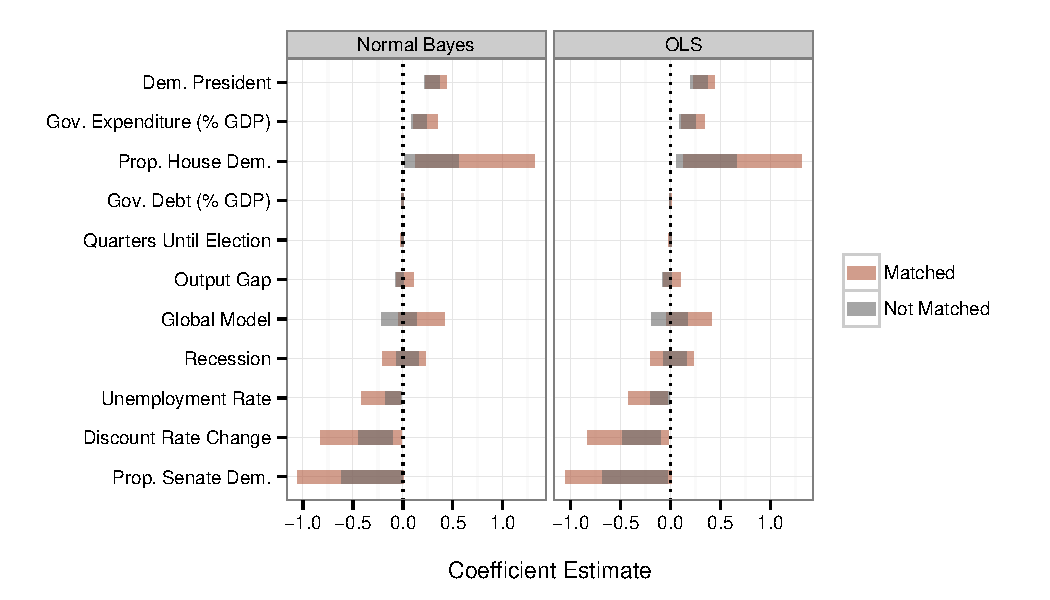
\includegraphics[width=0.95\linewidth]{figure/CoefComparePlots} 
\end{knitrout}

    \end{center}
    \begin{singlespace}
        {\scriptsize{Intercept values are not shown to maintain a reasonable scale for comparing covariate estimates.}}
    \end{singlespace}
\end{figure}

\paragraph{Presidential Party Identification}

Our main finding is that the--presidential party identification--had a strong positive association with Federal Reserve staff inflation forecast errors across all model specifications. This finding is what we would expect if Federal Reserve staff have a general presidential partisan bias and is very robust. For instance, the 95\% confidence band around the coefficient estimate moves somewhat further away from 0--i.e. no relationship--when using matched data (see Figure \ref{CoefComparePlots}).  

These analyses provide strong evidence that Federal Reserve staff overestimate the effect Democratic presidents have on inflation compared to Republican presidents.

\begin{figure}[t]
    \caption{Simulated Expected Inflation Forecast Error for Republican and Democratic Presidencies}
    \label{ExpectValueParty}
    \begin{center}

\begin{knitrout}
\definecolor{shadecolor}{rgb}{0.969, 0.969, 0.969}\color{fgcolor}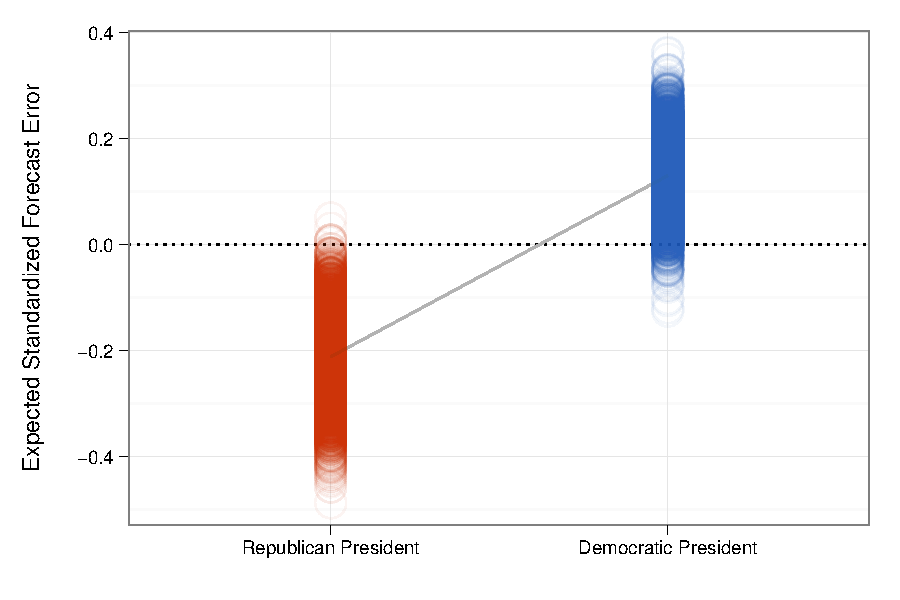
\includegraphics[width=0.7\linewidth]{figure/ExpectValueParty} 
\end{knitrout}

    \end{center}
    \begin{singlespace}
        {\scriptsize{From an OLS regression with data matched by presidential party identification. Variables included are the same as those in Model C6 from Table \ref{OutputPL}. \\ The figures show 1000 simulations per fitted value. \\ The solid line connects the two groups' means.}}
    \end{singlespace}
\end{figure}

To get a sense of approximately how big this bias might be we simulated expected standardized forecast errors for Democratic and Republican presidencies, holding all other covariates at their means.\footnote{1000 simulations were run on a normal Bayesian linear regression model matched by presidential party ID and including the same variables as those in Model C6 from Table \ref{OutputPL}.} Results from these simulations can be found in Figure \ref{ExpectValueParty}. We expect that on average the Fed overestimates inflation by 14 percent during Democratic presidencies. Expected average inflation error during Republican presidencies of -20 percent during Republican presidencies. Clearly, at least between 1970 and 2005, Fed staff were overly pessimistic about Democratic presidents' effect on inflation and even more overly optimistic about Republican presidents' effect. 

The estimated effects hold even when we control for actual government expenditure. This suggests that Federal Reserve staff are not simply responding to different levels of government spending that Democratic and Republican presidents may tend to initiate.

\paragraph{Presidential Elections}

We did not find any evidence that inflation forecast errors were associated with elections. This was true in parametric models using both unmatched data and matched data where the election period variable is the treatment. Estimates of the relationship between the quarters until election variable and forecast errors\footnote{This variable was obviously omitted from the models with the election period variable because they are highly correlated.} also did not provide any evidence that inflation errors are related to elections. 

Data limitations make it difficult to fully examine the extension of Clark and Arel-Bundock's \citeyearpar{Clark2011} election gaming approach to Federal Reserves staff.\footnote{We only have three Democratic presidential terms in our data, only two of which ended in the incumbent running for reelection.} Nonetheless, we attempted to examine this hypothesis with an interaction (not shown) of the president's party ID variable and both the election dummy and quarters to election variables. In all cases the president's party ID variable was robust whereas the election variables and the interaction term were very statistically insignificant. 

In this limited data set Fed Staff do not appear to be over estimating inflation when a Democratic president is running for reelection in an attempt to influence the FOMC to raise interest rates and lower the president's chances of winning. These findings have clear implications for how we understand the potential causes of Green Book partisan inflation forecast biases as well as FOMC interest rate decisions around elections. It seems that FOMC members, not their staff, are driving the increases in the Fed Funds Rate around elections when Democrats are in power that Clark and Arel-Bundock observed. 

\paragraph{Partisan Control of Congress}

Might Federal Reserve staff be taking into consideration not only the president's party identification, but also the partisan composition of Congress?  Across all of our datasets and parametric model specifications we find no evidence that the partisan composition of congressional chambers is related to inflation forecast errors. 

%%%%%%% President/Congress Interaction Plot %%%%%%%%
\begin{figure}[t]
    \caption{Simulated Interactions between President Party ID and Congressional Party Controls}
    \label{InterPlot}
    \begin{center}

\begin{knitrout}
\definecolor{shadecolor}{rgb}{0.969, 0.969, 0.969}\color{fgcolor}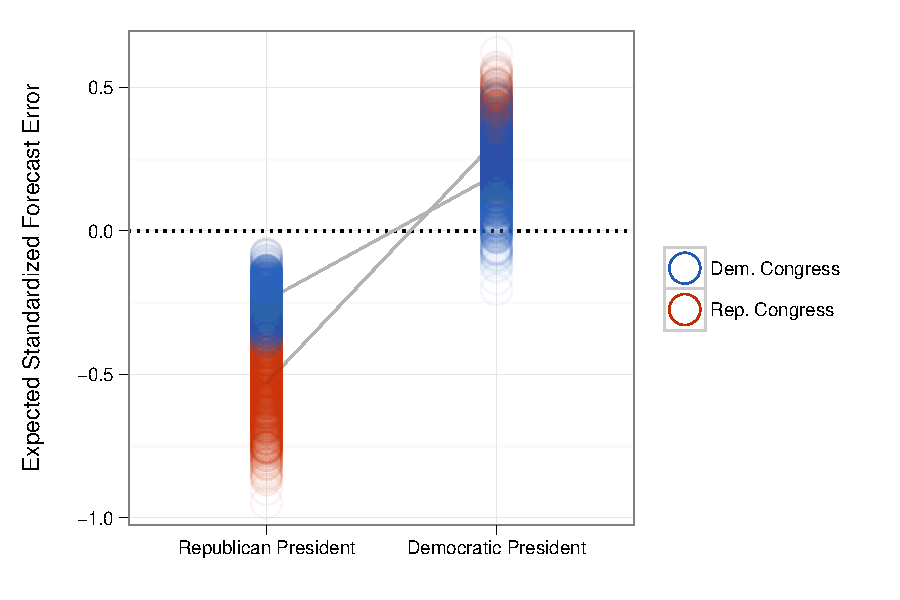
\includegraphics[width=0.8\linewidth]{figure/InterPlot} 
\end{knitrout}


    \end{center}
    \begin{singlespace}
        {\scriptsize{From an OLS regression with data matched by presidential party identification. Variables included are the same as those in Model C10 from Table \ref{OutputPL}. The figure show 1000 simulations per fitted value. \\ Both the House and Senate Democratic/Republican variables were set at 1.2 for Democratic congresses and 0.8 for Republican congresses. \\ The solid line connects the means of the congressional partisan control groups.}}
    \end{singlespace}
\end{figure}

We created parametric models with two-way and three-way interactions between presidential and congressional party identification to examine the two other ways we identified that presidential and congressional partisan ID might be related to forecast errors. All of the partisan interactions were generally statistically significant. To make substantive sense of these estimated interactions we use simulations, as above, to find expected inflation forecast errors at various levels of the presidential and congressional party identification. To highlight the findings, Figure \ref{InterPlot} shows the results of simulations where the levels of partisan convergence and divergence are at their most extreme: one party control of all bodies compared to a situation where different parties control the presidency and Congress.\footnote{Both the House and Senate Democratic/Republican variables were set at 1.2 for Democratic congresses and 0.8 for Republican congresses.} 

The first thing we should notice in Figure \ref{InterPlot} is how presidential partisan identification still seems to be driving the direction of the inflation forecast error: inflation is underestimated during Republican presidencies and overestimated during Democratic ones, regardless of partisan control in Congress. The estimated substantive effect of congressional control on forecast errors in the magnitude of the over or under estimates. In particular, inflation is very underestimated for Republican presidencies with Republican congresses. There may be an expectation among Fed Staff that these governments will cut expenditure much more than they actually do. Forecast error is slightly higher on average with Democratic presidencies and Republican congresses compared to when both are controlled by Democrats. This finding fits with a story where Fed Staff believe spending will be higher with a divided government. However the difference between the two means is small\footnote{There is a 12 percentage point difference between the two.} and there is considerable overlap in the two groups of simulation results.

Despite some evidence for an interaction between congressional and presidential party identification, it is not clear at this time how these results can be consistently explained across Democratic and Republican presidencies. 

\paragraph{Government Expenditure}

Nonetheless, it seems that Federal Reserve staff may also overestimate the effect of government expenditure on inflation. This is indicated by a consistently positive and significant coefficient for the government expenditure variable, even when controlling for president's party ID. 

\paragraph{FRB Global Forecasting Model}

The introduction of the FRB/Global behavioral equation forecasting model does not seem to have begun an era of significantly lower inflation forecasting error. In fact, across all of our matching and parametric model specifications, forecasts made after the introduction of this approach are not significantly different than those made before it. 

\paragraph{Changes to the Discount Rate}

As expected, relative changes to the discount rate were often found to be negatively associated with inflation forecast errors. Increasing the discount rate could result in lower inflation than expected and vice versa. Controlling for FOMC policy did not affect the estimated relationship between presidential party ID and errors. Also, the results were not robust across all of the models. 

\section*{Discussion: Do Fed Forecasts Have a Partisan Bias?}

FILL IN

MAYBE TALK ABOUT HOW IT IS STRANGE THAT ACTORS WITH ``RATIONAL" PARTISAN EXPECTATIONS WOULD NOT UPDATE THEIR INFLATION EXPECTATIONS. I.E. WHY WOULD THEY CONTINUE TO BE WRONG ABOUT INFLATION GIVEN THE PRESIDENT'S PARTY ID?

\clearpage
\section*{Appendix}

\subsection*{Replication}

This paper was written with {\tt{knitr}} \citep{knitr2012}. It can be entirely replicated from data, analysis source code, and markup files available as a {\tt{.zip}} file downloadable from our GitHub page at: {\url{https://github.com/christophergandrud/GreenBook/zipball/master}}. 

%%%%%%% Table of non-matched data with OLS parametric model %%%%%%%%

\begin{table}[ht]
    \caption{OLS Estimation of Covariate Effects on 2 Qtr. Inflation Forecast Error (non-matched dataset)}
    \label{OutputNL}
    \vspace{0.25cm}
    \begin{center}
    {\footnotesize

 
\begin{tabular}{ l D{.}{.}{1}D{.}{.}{1}D{.}{.}{1}D{.}{.}{1}D{.}{.}{1}D{.}{.}{1}D{.}{.}{1}D{.}{.}{1}D{.}{.}{1}D{.}{.}{1}D{.}{.}{1}D{.}{.}{1} } 
\hline 
  & \multicolumn{ 1 }{ c }{ A1 } & \multicolumn{ 1 }{ c }{ A2 } & \multicolumn{ 1 }{ c }{ A3 } & \multicolumn{ 1 }{ c }{ A4 } & \multicolumn{ 1 }{ c }{ A5 } & \multicolumn{ 1 }{ c }{ A6 } & \multicolumn{ 1 }{ c }{ A7 } & \multicolumn{ 1 }{ c }{ A8 } & \multicolumn{ 1 }{ c }{ A9 } & \multicolumn{ 1 }{ c }{ A10 } & \multicolumn{ 1 }{ c }{ A11 } & \multicolumn{ 1 }{ c }{ A12 } \\ \hline
 %                    & A1             & A2             & A3             & A4             & A5             & A6             & A7             & A8             & A9             & A10            & A11            & A12           \\ 
Intercept            & 3.3 ^{**}      & 3.6 ^{**}      & 3.3 ^{**}      & 4.3 ^{***}     & 4.5 ^{***}     & 4.6 ^{***}     & 4.6 ^{***}     & 4.8 ^{***}     & 4.4 ^{***}     & 4.0 ^{***}     & 2.3 ^\dagger  & -2.2 ^{***}   \\ 
                     & (1.1)          & (1.2)          & (1.1)          & (0.9)          & (1.0)          & (1.0)          & (1.0)          & (1.0)          & (0.9)          & (0.9)          & (1.2)          & (0.4)         \\ 
Recession            & -0.0           & -0.0           & -0.0           & 0.0            & 0.1            & 0.1            & 0.1            & 0.1            & 0.1 ^\dagger  & 0.1            & 0.1            &               \\ 
                     & (0.1)          & (0.1)          & (0.1)          & (0.0)          & (0.1)          & (0.1)          & (0.1)          & (0.1)          & (0.0)          & (0.0)          & (0.0)          &               \\ 
Debt/GDP             & 0.0            & 0.0            & 0.0            & -0.0 ^*        & -0.0 ^*        & -0.0           & 0.0            & -0.0           & -0.0           & -0.0           & 0.0            &               \\ 
                     & (0.0)          & (0.0)          & (0.0)          & (0.0)          & (0.0)          & (0.0)          & (0.0)          & (0.0)          & (0.0)          & (0.0)          & (0.0)          &               \\ 
Expenditure/GDP      & 0.1 ^{***}     & 0.1 ^{***}     & 0.1 ^{***}     & 0.2 ^{***}     & 0.2 ^{***}     & 0.2 ^{***}     & 0.1 ^{***}     & 0.2 ^{***}     & 0.1 ^{***}     & 0.2 ^{***}     & 0.1 ^{***}     &               \\ 
                     & (0.0)          & (0.0)          & (0.0)          & (0.0)          & (0.0)          & (0.0)          & (0.0)          & (0.0)          & (0.0)          & (0.0)          & (0.0)          &               \\ 
Output Gap           & -0.1 ^{***}    & -0.1 ^{***}    & -0.1 ^{***}    & -0.1 ^{***}    & -0.1 ^{***}    & -0.1 ^{***}    & -0.1 ^{***}    & -0.1 ^{***}    & -0.1 ^{***}    & -0.1 ^{***}    & -0.1 ^{***}    &               \\ 
                     & (0.0)          & (0.0)          & (0.0)          & (0.0)          & (0.0)          & (0.0)          & (0.0)          & (0.0)          & (0.0)          & (0.0)          & (0.0)          &               \\ 
Discount Rate Change & -0.0           & -0.0           & -0.0           & -0.2 ^{**}     & -0.2 ^{**}     & -0.2 ^{**}     & -0.2 ^{**}     & -0.3 ^{**}     & -0.2 ^*        & -0.2 ^*        & -0.2 ^*        &               \\ 
                     & (0.1)          & (0.1)          & (0.1)          & (0.1)          & (0.1)          & (0.1)          & (0.1)          & (0.1)          & (0.1)          & (0.1)          & (0.1)          &               \\ 
Qtr. to Election     &                & -0.0           &                &                & -0.0           & -0.0           & -0.0           & -0.0           & 0.0            & 0.0            & 0.0            &               \\ 
                     &                & (0.0)          &                &                & (0.0)          & (0.0)          & (0.0)          & (0.0)          & (0.0)          & (0.0)          & (0.0)          &               \\ 
Election Period      &                &                & 0.0            &                &                &                &                &                &                &                &                &               \\ 
                     &                &                & (0.1)          &                &                &                &                &                &                &                &                &               \\ 
Pres. Party ID       &                &                &                & 0.3 ^{***}     & 0.3 ^{***}     & 0.3 ^{***}     & 0.3 ^{***}     & 0.3 ^{***}     & 1.0 ^{***}     & 1.1 ^{***}     & 2.2 ^{***}     & 2.6 ^{***}    \\ 
                     &                &                &                & (0.0)          & (0.0)          & (0.0)          & (0.0)          & (0.0)          & (0.1)          & (0.2)          & (0.6)          & (0.7)         \\ 
Senate Dem/Rep       &                &                &                &                &                & -0.1           & -0.2           &                & -0.1           & -0.0           & 0.8 ^*         & 1.1 ^{***}    \\ 
                     &                &                &                &                &                & (0.1)          & (0.2)          &                & (0.1)          & (0.1)          & (0.3)          & (0.3)         \\ 
House Dem/Rep        &                &                &                &                &                & 0.1            & 0.2            &                & 0.4 ^{**}      & 0.3 ^*         & 1.2 ^{***}     & 1.8 ^{***}    \\ 
                     &                &                &                &                &                & (0.1)          & (0.1)          &                & (0.1)          & (0.1)          & (0.3)          & (0.3)         \\ 
FRB/GlobalModel      &                &                &                &                &                &                & -0.1           &                &                &                &                &               \\ 
                     &                &                &                &                &                &                & (0.1)          &                &                &                &                &               \\ 
Greenspan            &                &                &                &                &                &                &                & -0.1           &                &                &                &               \\ 
                     &                &                &                &                &                &                &                & (0.1)          &                &                &                &               \\ 
Martin               &                &                &                &                &                &                &                & 0.0            &                &                &                &               \\ 
                     &                &                &                &                &                &                &                & (0.1)          &                &                &                &               \\ 
Miller               &                &                &                &                &                &                &                & -0.1           &                &                &                &               \\ 
                     &                &                &                &                &                &                &                & (0.1)          &                &                &                &               \\ 
Volcker              &                &                &                &                &                &                &                & -0.0           &                &                &                &               \\ 
                     &                &                &                &                &                &                &                & (0.1)          &                &                &                &               \\ 
Pres Party ID*House  &                &                &                &                &                &                &                &                & -0.5 ^{***}    &                & -1.8 ^*        & -2.6 ^{**}    \\ 
                     &                &                &                &                &                &                &                &                & (0.1)          &                & (0.8)          & (0.8)         \\ 
Pres Party ID*Senate &                &                &                &                &                &                &                &                &                & -0.7 ^{***}    & -0.8           & -0.6          \\ 
                     &                &                &                &                &                &                &                &                &                & (0.1)          & (0.7)          & (0.6)         \\ 
House*Senate         &                &                &                &                &                &                &                &                &                &                & -0.6 ^{**}     & -1.0 ^{***}   \\ 
                     &                &                &                &                &                &                &                &                &                &                & (0.2)          & (0.2)         \\ 
Pres*House*Senate    &                &                &                &                &                &                &                &                &                &                & 0.8 ^\dagger  & 1.2 ^*        \\ 
                     &                &                &                &                &                &                &                &                &                &                & (0.4)          & (0.5)          \\
 $N$                  & 148            & 148            & 148            & 148            & 148            & 148            & 148            & 148            & 148            & 148            & 148            & 148           \\ 
$R^2$                & 0.3            & 0.3            & 0.3            & 0.5            & 0.5            & 0.5            & 0.5            & 0.5            & 0.6            & 0.6            & 0.6            & 0.5           \\ 
adj. $R^2$           & 0.2            & 0.2            & 0.2            & 0.5            & 0.5            & 0.5            & 0.5            & 0.5            & 0.6            & 0.6            & 0.6            & 0.5           \\ 
Resid. sd            & 0.2            & 0.2            & 0.2            & 0.2            & 0.2            & 0.2            & 0.2            & 0.2            & 0.2            & 0.2            & 0.2            & 0.2            \\ \hline
 \multicolumn{13}{l}{\footnotesize{Standard errors in parentheses}}\\
\multicolumn{13}{l}{\footnotesize{$^\dagger$ significant at $p<.10$; $^* p<.05$; $^{**} p<.01$; $^{***} p<.001$}} 
\end{tabular} 



    }
    \end{center}
\end{table}

%%%%%%% Table of ElectionPeriod matched data with OLS parametric model %%%%%%%%

\begin{table}[ht]
    \caption{OLS Estimation of Covariate Effects on 2 Qtr. Inflation Forecast Error (Matched by Election Period Variable)}
    \label{OutputEL}
    \vspace{0.25cm}
    \begin{center}
    {\footnotesize

 
\begin{tabular}{ l D{.}{.}{1}D{.}{.}{1}D{.}{.}{1}D{.}{.}{1}D{.}{.}{1}D{.}{.}{1}D{.}{.}{1}D{.}{.}{1}D{.}{.}{1}D{.}{.}{1}D{.}{.}{1} } 
\hline 
  & \multicolumn{ 1 }{ c }{ B1 } & \multicolumn{ 1 }{ c }{ B2 } & \multicolumn{ 1 }{ c }{ B3 } & \multicolumn{ 1 }{ c }{ B4 } & \multicolumn{ 1 }{ c }{ B5 } & \multicolumn{ 1 }{ c }{ B6 } & \multicolumn{ 1 }{ c }{ B7 } & \multicolumn{ 1 }{ c }{ B8 } & \multicolumn{ 1 }{ c }{ B9 } & \multicolumn{ 1 }{ c }{ B10 } & \multicolumn{ 1 }{ c }{ B11 } \\ \hline
 %                    & B1              & B2              & B3              & B4              & B5              & B6              & B7              & B8              & B9              & B10             & B11            \\ 
Intercept            & 1.7             & 2.2             & 1.6             & 1.7             & 2.0             & 2.5             & 1.9             & 0.3             & -0.6            & 1.5             & -2.2 ^{**}     \\ 
                     & (2.8)           & (2.8)           & (2.8)           & (2.4)           & (2.5)           & (2.9)           & (4.0)           & (2.4)           & (2.6)           & (4.7)           & (0.6)          \\ 
Debt/GDP             & 0.0             & 0.0             & 0.0             & -0.0            & -0.0            & 0.0             & 0.0             & -0.0 ^\dagger  & -0.0 ^*         & 0.0             &                \\ 
                     & (0.0)           & (0.0)           & (0.0)           & (0.0)           & (0.0)           & (0.0)           & (0.0)           & (0.0)           & (0.0)           & (0.0)           &                \\ 
Expenditure/GDP      & 0.1 ^*          & 0.1 ^*          & 0.1 ^*          & 0.2 ^{***}      & 0.2 ^{***}      & 0.1 ^*          & 0.1             & 0.3 ^{***}      & 0.3 ^{***}      & 0.1             &                \\ 
                     & (0.0)           & (0.0)           & (0.0)           & (0.0)           & (0.0)           & (0.1)           & (0.1)           & (0.1)           & (0.1)           & (0.1)           &                \\ 
Output Gap           & -0.0            & -0.0            & -0.0            & -0.1 ^\dagger  & -0.1 ^\dagger  & -0.1            & -0.0            & -0.1 ^\dagger  & -0.1            & -0.0            &                \\ 
                     & (0.0)           & (0.0)           & (0.0)           & (0.0)           & (0.0)           & (0.0)           & (0.1)           & (0.0)           & (0.0)           & (0.0)           &                \\ 
Discount Rate Change & -0.7 ^{**}      & -0.7 ^*         & -0.7 ^{**}      & -0.5 ^*         & -0.5 ^\dagger  & -0.4            & -0.4            & -0.2            & -0.1            & -0.2            &                \\ 
                     & (0.3)           & (0.3)           & (0.2)           & (0.2)           & (0.2)           & (0.3)           & (0.4)           & (0.2)           & (0.2)           & (0.3)           &                \\ 
Qtr. to Election     &                 & -0.0            &                 &                 & -0.0            & -0.0            & -0.0            & -0.0            & -0.0            & -0.0            &                \\ 
                     &                 & (0.0)           &                 &                 & (0.0)           & (0.0)           & (0.0)           & (0.0)           & (0.0)           & (0.0)           &                \\ 
Election Period      &                 &                 & 0.1             &                 &                 &                 &                 &                 &                 &                 &                \\ 
                     &                 &                 & (0.1)           &                 &                 &                 &                 &                 &                 &                 &                \\ 
Pres. Party ID       &                 &                 &                 & 0.3 ^{**}       & 0.3 ^{**}       & 0.3 ^*          & 0.3 ^*          & 1.3 ^{***}      & 1.7 ^{***}      & 20.9            & 25.0           \\ 
                     &                 &                 &                 & (0.1)           & (0.1)           & (0.1)           & (0.1)           & (0.3)           & (0.5)           & (23.8)          & (17.7)         \\ 
Senate Dem/Rep       &                 &                 &                 &                 &                 & -0.1            & -0.1            & 0.3             & 0.5 ^\dagger   & 0.4             & 0.9            \\ 
                     &                 &                 &                 &                 &                 & (0.3)           & (0.4)           & (0.3)           & (0.3)           & (0.8)           & (0.6)          \\ 
House Dem/Rep        &                 &                 &                 &                 &                 & 0.2             & 0.2             & -0.2            & -0.4            & 1.0             & 1.8 ^{***}     \\ 
                     &                 &                 &                 &                 &                 & (0.3)           & (0.3)           & (0.3)           & (0.3)           & (0.8)           & (0.4)          \\ 
FRB/GlobalModel      &                 &                 &                 &                 &                 &                 & -0.1            &                 &                 &                 &                \\ 
                     &                 &                 &                 &                 &                 &                 & (0.3)           &                 &                 &                 &                \\ 
Pres Party ID*House  &                 &                 &                 &                 &                 &                 &                 & -0.8 ^{**}      &                 & -21.8           & -26.3          \\ 
                     &                 &                 &                 &                 &                 &                 &                 & (0.2)           &                 & (23.4)          & (16.7)         \\ 
Pres Party ID*Senate &                 &                 &                 &                 &                 &                 &                 &                 & -1.3 ^{**}      & -14.3           & -17.0          \\ 
                     &                 &                 &                 &                 &                 &                 &                 &                 & (0.4)           & (19.2)          & (14.7)         \\ 
House*Senate         &                 &                 &                 &                 &                 &                 &                 &                 &                 & -0.4            & -0.9 ^{**}     \\ 
                     &                 &                 &                 &                 &                 &                 &                 &                 &                 & (0.5)           & (0.3)          \\ 
Pres*House*Senate    &                 &                 &                 &                 &                 &                 &                 &                 &                 & 15.2            & 18.2           \\ 
                     &                 &                 &                 &                 &                 &                 &                 &                 &                 & (17.9)          & (13.0)          \\
 $N$                  & 32              & 32              & 32              & 32              & 32              & 32              & 32              & 32              & 32              & 32              & 32             \\ 
$R^2$                & 0.5             & 0.5             & 0.5             & 0.6             & 0.6             & 0.6             & 0.6             & 0.8             & 0.8             & 0.8             & 0.7            \\ 
adj. $R^2$           & 0.4             & 0.4             & 0.4             & 0.6             & 0.5             & 0.5             & 0.5             & 0.7             & 0.7             & 0.7             & 0.7            \\ 
Resid. sd            & 0.2             & 0.2             & 0.2             & 0.2             & 0.2             & 0.2             & 0.2             & 0.1             & 0.2             & 0.2             & 0.2             \\ \hline
 \multicolumn{12}{l}{\footnotesize{Standard errors in parentheses}}\\
\multicolumn{12}{l}{\footnotesize{$^\dagger$ significant at $p<.10$; $^* p<.05$; $^{**} p<.01$; $^{***} p<.001$}}\\
\multicolumn{12}{l}{\footnotesize{The recession variable is ommitted because there was no variation in the matched data set.}}\\
\multicolumn{12}{l}{\footnotesize{The reason that there was no variation is because there was never a recession during an}}\\
\multicolumn{12}{l}{\footnotesize{election period in our data set.}} 
\end{tabular} 



    }
    \end{center}
\end{table}

%%%%%%% Table of pres_party matched data with OLS parametric model %%%%%%%%

\begin{table}[ht]
    \caption{OLS Estimation of Covariate Effects on 2 Qtr. Inflation Forecast Error (Matched by President's Party ID variable)}
    \label{OutputPL}
    \vspace{0.25cm}
    \begin{center}
    {\footnotesize

 
\begin{tabular}{ l D{.}{.}{1}D{.}{.}{1}D{.}{.}{1}D{.}{.}{1}D{.}{.}{1}D{.}{.}{1}D{.}{.}{1}D{.}{.}{1}D{.}{.}{1}D{.}{.}{1}D{.}{.}{1} } 
\hline 
  & \multicolumn{ 1 }{ c }{ C1 } & \multicolumn{ 1 }{ c }{ C2 } & \multicolumn{ 1 }{ c }{ C3 } & \multicolumn{ 1 }{ c }{ C4 } & \multicolumn{ 1 }{ c }{ C5 } & \multicolumn{ 1 }{ c }{ C6 } & \multicolumn{ 1 }{ c }{ C7 } & \multicolumn{ 1 }{ c }{ C8 } & \multicolumn{ 1 }{ c }{ C9 } & \multicolumn{ 1 }{ c }{ C10 } & \multicolumn{ 1 }{ c }{ C11 } \\ \hline
 %                    & C1              & C2              & C3              & C4              & C5              & C6              & C7              & C8              & C9              & C10             & C11            \\ 
Intercept            & 4.6             & 4.6             & 4.5             & 7.2 ^*          & 7.2 ^*          & 5.9 ^\dagger   & 5.8 ^\dagger   & 3.3             & 2.5             & 2.1             & -2.4 ^{**}     \\ 
                     & (3.5)           & (3.5)           & (3.5)           & (2.9)           & (2.9)           & (3.1)           & (3.1)           & (2.6)           & (2.7)           & (3.3)           & (0.7)          \\ 
Recession            & 0.1             & 0.1             & 0.1             & 0.2 ^\dagger   & 0.2 ^\dagger   & 0.2             & 0.2             & 0.1             & 0.1             & 0.1             &                \\ 
                     & (0.1)           & (0.1)           & (0.1)           & (0.1)           & (0.1)           & (0.1)           & (0.1)           & (0.1)           & (0.1)           & (0.1)           &                \\ 
Debt/GDP             & 0.0             & 0.0             & 0.0             & -0.0            & -0.0            & -0.0            & -0.0            & -0.0            & -0.0            & -0.0            &                \\ 
                     & (0.0)           & (0.0)           & (0.0)           & (0.0)           & (0.0)           & (0.0)           & (0.0)           & (0.0)           & (0.0)           & (0.0)           &                \\ 
Expenditure/GDP      & 0.1 ^*          & 0.1 ^*          & 0.1 ^*          & 0.2 ^{***}      & 0.2 ^{***}      & 0.2 ^{**}       & 0.2 ^{**}       & 0.2 ^{**}       & 0.2 ^{***}      & 0.1 ^\dagger   &                \\ 
                     & (0.1)           & (0.1)           & (0.1)           & (0.1)           & (0.1)           & (0.1)           & (0.1)           & (0.1)           & (0.1)           & (0.1)           &                \\ 
Output Gap           & -0.1            & -0.1            & -0.1            & -0.1 ^{**}      & -0.1 ^{**}      & -0.1 ^*         & -0.1 ^*         & -0.1 ^*         & -0.1 ^\dagger  & -0.1            &                \\ 
                     & (0.0)           & (0.0)           & (0.0)           & (0.0)           & (0.0)           & (0.0)           & (0.0)           & (0.0)           & (0.0)           & (0.0)           &                \\ 
Discount Rate Change & -0.2            & -0.1            & -0.1            & -0.5 ^\dagger  & -0.5 ^\dagger  & -0.4            & -0.4            & -0.2            & -0.1            & -0.2            &                \\ 
                     & (0.3)           & (0.3)           & (0.3)           & (0.3)           & (0.3)           & (0.3)           & (0.3)           & (0.2)           & (0.2)           & (0.2)           &                \\ 
Qtr. to Election     &                 & -0.0            &                 &                 & -0.0            & 0.0             & 0.0             & 0.0 ^\dagger   & 0.0             & 0.0             &                \\ 
                     &                 & (0.0)           &                 &                 & (0.0)           & (0.0)           & (0.0)           & (0.0)           & (0.0)           & (0.0)           &                \\ 
Election Period      &                 &                 & 0.0             &                 &                 &                 &                 &                 &                 &                 &                \\ 
                     &                 &                 & (0.1)           &                 &                 &                 &                 &                 &                 &                 &                \\ 
Pres. Party ID       &                 &                 &                 & 0.3 ^{***}      & 0.3 ^{***}      & 0.3 ^{***}      & 0.3 ^{***}      & 1.4 ^{***}      & 1.5 ^{***}      & 2.3 ^*          & 2.9 ^{**}      \\ 
                     &                 &                 &                 & (0.1)           & (0.1)           & (0.1)           & (0.1)           & (0.2)           & (0.3)           & (1.0)           & (0.9)          \\ 
Senate Dem/Rep       &                 &                 &                 &                 &                 & -0.3            & -0.3            & -0.1            & 0.1             & 0.5             & 1.1            \\ 
                     &                 &                 &                 &                 &                 & (0.2)           & (0.3)           & (0.2)           & (0.2)           & (0.8)           & (0.7)          \\ 
House Dem/Rep        &                 &                 &                 &                 &                 & 0.0             & 0.0             & 0.5 ^{**}       & 0.3 ^\dagger   & 1.2 ^\dagger   & 1.9 ^{***}     \\ 
                     &                 &                 &                 &                 &                 & (0.2)           & (0.2)           & (0.2)           & (0.2)           & (0.7)           & (0.5)          \\ 
FRB/GlobalModel      &                 &                 &                 &                 &                 &                 & 0.0             &                 &                 &                 &                \\ 
                     &                 &                 &                 &                 &                 &                 & (0.1)           &                 &                 &                 &                \\ 
Pres Party ID*House  &                 &                 &                 &                 &                 &                 &                 & -0.8 ^{***}     &                 & -2.0 ^\dagger  & -2.8 ^{**}     \\ 
                     &                 &                 &                 &                 &                 &                 &                 & (0.2)           &                 & (1.0)           & (0.9)          \\ 
Pres Party ID*Senate &                 &                 &                 &                 &                 &                 &                 &                 & -1.0 ^{***}     & -0.5            & -0.6           \\ 
                     &                 &                 &                 &                 &                 &                 &                 &                 & (0.2)           & (1.3)           & (0.8)          \\ 
House*Senate         &                 &                 &                 &                 &                 &                 &                 &                 &                 & -0.5            & -1.0 ^*        \\ 
                     &                 &                 &                 &                 &                 &                 &                 &                 &                 & (0.5)           & (0.4)          \\ 
Pres*House*Senate    &                 &                 &                 &                 &                 &                 &                 &                 &                 & 0.7             & 1.1 ^\dagger  \\ 
                     &                 &                 &                 &                 &                 &                 &                 &                 &                 & (0.7)           & (0.6)           \\
 $N$                  & 68              & 68              & 68              & 68              & 68              & 68              & 68              & 68              & 68              & 68              & 68             \\ 
$R^2$                & 0.2             & 0.2             & 0.2             & 0.4             & 0.4             & 0.5             & 0.5             & 0.6             & 0.6             & 0.6             & 0.6            \\ 
adj. $R^2$           & 0.1             & 0.1             & 0.1             & 0.4             & 0.4             & 0.4             & 0.4             & 0.6             & 0.6             & 0.6             & 0.6            \\ 
Resid. sd            & 0.2             & 0.2             & 0.2             & 0.2             & 0.2             & 0.2             & 0.2             & 0.2             & 0.2             & 0.2             & 0.2             \\ \hline
 \multicolumn{12}{l}{\footnotesize{Standard errors in parentheses}}\\
\multicolumn{12}{l}{\footnotesize{$^\dagger$ significant at $p<.10$; $^* p<.05$; $^{**} p<.01$; $^{***} p<.001$}} 
\end{tabular} 



    }
    \end{center}
\end{table}

%%%%%%% Table of pres_party matched data with Bayesian normal linear parametric 

% latex table generated in R 2.15.1 by xtable 1.7-0 package
% Mon Jul 30 09:42:33 2012
\begin{table}[ht]
\begin{center}
\caption{Bayesian Normal Linear Regression Estimation of Covariate Effects on 2 Qtr. Inflation Forecast Error (non-matched data set)}
\label{OutputNB}
{\small
\begin{tabular}{lccccc}
  \hline
Variables & Mean & SD & 2.5\% & 50\% & 97.5\% \\ 
  \hline
Intercept & 4.60 & 1.00 & 2.66 & 4.59 & 6.57 \\ 
  Pres. Party ID & 0.29 & 0.04 & 0.21 & 0.29 & 0.37 \\ 
  Recession & 0.06 & 0.05 & -0.04 & 0.06 & 0.17 \\ 
  Qtr. to Election & -0.00 & 0.00 & -0.01 & -0.00 & 0.00 \\ 
  Senate Dem/Rep & -0.24 & 0.16 & -0.55 & -0.24 & 0.06 \\ 
  House Dem/Rep & 0.15 & 0.13 & -0.10 & 0.15 & 0.41 \\ 
  Debt/GDP & 0.00 & 0.00 & -0.01 & 0.00 & 0.01 \\ 
  Expenditure/GDP & 0.12 & 0.03 & 0.06 & 0.12 & 0.19 \\ 
  Output Gap & -0.07 & 0.01 & -0.10 & -0.07 & -0.05 \\ 
  Discount Rate Change & -0.24 & 0.09 & -0.42 & -0.24 & -0.07 \\ 
  Global Model & -0.09 & 0.08 & -0.26 & -0.09 & 0.07 \\ 
  sigma2 & 0.04 & 0.00 & 0.03 & 0.04 & 0.05 \\ 
   \hline
\end{tabular}
}
\end{center}
\end{table}





%%%%%%% Table of pres_party matched data with Normal Bayesian linear parametric model %%%%%%%%


% latex table generated in R 2.15.1 by xtable 1.7-0 package
% Mon Jul 30 09:42:34 2012
\begin{table}[ht]
\begin{center}
\caption{Bayesian Normal Linear Regression Estimation of Covariate Effects on 2 Qtr. Inflation Forecast Error (Matched by President's Party ID variable}
\label{OutputPB}
{\small
\begin{tabular}{lccccc}
  \hline
Variables & Mean & SD & 2.5\% & 50\% & 97.5\% \\ 
  \hline
Intercept & 5.84 & 3.20 & -0.42 & 5.83 & 12.09 \\ 
  Pres. Party ID & 0.34 & 0.07 & 0.21 & 0.34 & 0.47 \\ 
  Recession & 0.16 & 0.11 & -0.06 & 0.16 & 0.39 \\ 
  Qtr. to Election & 0.00 & 0.01 & -0.01 & 0.00 & 0.02 \\ 
  Senate Dem/Rep & -0.31 & 0.28 & -0.85 & -0.31 & 0.24 \\ 
  House Dem/Rep & 0.02 & 0.21 & -0.40 & 0.02 & 0.42 \\ 
  Debt/GDP & -0.01 & 0.01 & -0.02 & -0.01 & 0.00 \\ 
  Expenditure/GDP & 0.22 & 0.07 & 0.08 & 0.22 & 0.35 \\ 
  Output Gap & -0.10 & 0.04 & -0.18 & -0.10 & -0.02 \\ 
  Discount Rate Change & -0.36 & 0.28 & -0.90 & -0.36 & 0.19 \\ 
  Global Model & 0.02 & 0.13 & -0.23 & 0.02 & 0.27 \\ 
  sigma2 & 0.04 & 0.01 & 0.03 & 0.04 & 0.06 \\ 
   \hline
\end{tabular}
}
\end{center}
\end{table}




%%%%%%% References %%%%%%%%%%%%

\clearpage

\bibliographystyle{apsr}
\bibliography{GreenBook.bib}

\end{document}
